% arara: clean: {
% arara: --> extensions:
% arara: --> ['aux', 'log', 'out', 'pdf']
% arara: --> }
%! arara: lualatex: {
%! arara: --> shell: yes,
%! arara: --> draft: yes,
%! arara: --> interaction: batchmode
%! arara: --> }
%! arara: biber
% arara: lualatex: {
% arara: --> shell: yes,
% arara: --> draft: no,
% arara: --> interaction: batchmode
% arara: --> }
% arara: lualatex: {
% arara: --> shell: yes,
% arara: --> draft: no,
% arara: --> interaction: batchmode
% arara: --> }
% arara: clean: {
% arara: --> extensions:
% arara: --> ['aux', 'log', 'out']
% arara: --> }
\documentclass[
	12pt,
	oneside,
	appendixprefix=true
]{scrbook}
\usepackage[spanish]{babel}
\decimalpoint
\usepackage{diffcoeff}
\usepackage[intlimits]{mathtools}
\usepackage{amssymb}
\usepackage{amsthm}
\usepackage{graphicx}
\usepackage{minted}
\usepackage[
	citestyle=numeric,
	style=numeric,
	backend=biber,
]{biblatex}
\usepackage{hyperref}

\title{
	Una introducción acerca de los métodos de volúmenes finitos para
	una ecuación de transporte
}
\author{\scshape\name}
\date{\today}

% \addtokomafont{section}{\centering}
% \addtokomafont{subsection}{\centering}

\theoremstyle{definition}
\newtheorem{theorem}{Teorema}
\newtheorem{definition}{Definición}
\newtheorem{remark}{Observación}
\newtheorem{example}{Ejemplo}
\addbibresource{references.bib}

\providecommand{\name}{Carlos Aznarán} % Nombre
\renewcommand{\listingscaption}{Programa}
\renewcommand{\listoflistingscaption}{Lista de \listingscaption s}

\hypersetup{
	pdfencoding=auto,
	linktocpage=true,
	colorlinks=true,
	linkcolor=blue,
	urlcolor=magenta,
	pdfpagelabels,
	pdftex,
	pdfauthor={Carlos Aznarán Laos},
	pdftitle={Una introducción acerca de los métodos de volúmenes
			finitos para una ecuación de transporte},
	pdfsubject={Lecture},
	pdfkeywords={finite volume, pde, transport equation},
	pdfproducer={LuaHBTeX, Version 1.18.0 (TeX Live 2024/Arch Linux)},
	% bookmark=false
}

\clearpage
\pagestyle{empty}
\renewcommand*{\chapterpagestyle}{empty}

\begin{document}

\providecommand{\faculty}{Facultad}
\noindent\parbox[c]{.18\textwidth}{
\includegraphics[width=2.8cm]{logouni}}\hfill
\parbox[c]{1\textwidth}{\raggedright%
    {\large\textbf{UNIVERSIDAD NACIONAL DE INGENIERÍA} \par\smallskip}
    {\large\textbf{\faculty} \par\smallskip}
    {\large\textbf{DEPARTAMENTO ACADÉMICO DE CIENCIAS BÁSICAS} \par\smallskip}
}

\begin{center}\bfseries\large
    Práctica Dirigida 3 de Métodos Numéricos (BMA-18)
    Parte $2$
\end{center}

\vspace{-0.5cm}

\hrulefill
\vspace{-2.5mm}

\rule{16.5cm}{0.8mm}

\section{Semana 4}

\subsection{Ecuaciones Diferenciales Ordinarias}

Una ecuación diferencial es una ecuación que involucra sus derivadas.
En la forma
\begin{equation*}
    \diff{y}{t}=f\left(t,y\left(t\right)\right),
\end{equation*}
Una ecuación diferencial de primer orden expresa la tasa de cambio de
una cantidad $y$ en términos del tiempo presente y el valor actual de
la cantidad.
Las ecuaciones diferenciales se utilizan para modelar, comprender y
predecir sistemas que cambian con el tiempo.
Para aproximar las soluciones de una ecuación diferencial ordinaria
(EDO) por métodos computacionales, veremos el método de Euler,
métodos implícitos y multipasos.

\subsection{Método de Euler explícito}

Para mostrar una implementación del método de seguimiento
computacional del campo de pendientes, empezemos con una cuadrícula
de $n+1$ puntos
\begin{equation*}
    t_{0}<t_{1}<t_{2}<\cdots<t_{n}
\end{equation*}
a lo largo del eje $t$ con un tamaño de constante igual a $h$.
Comience con $w_{0}=y_{0}$.
Siguiendo el campo de pendientes en cada $t_{i}$ se obtiene la
aproximación
\begin{equation*}
    w_{i+1}=w_{i}+hf\left(t_{i},w_{i}\right)
\end{equation*}
en $t_{i+1}$, ya que $f\left(t_{i},w_{i}\right)$ representa la
pendiente de la solución.
Nótese que el cambio en $y$ es la distancia horizontal $h$
multiplicada por la pendiente.
Así, cada $w_{i}$ es una aproximación de la solución en $t_{i}$.

\begin{figure}[ht!]
    \centering
    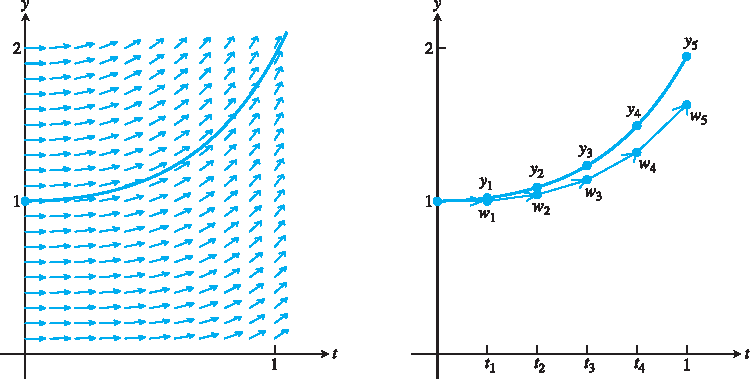
\includegraphics[width=.6\paperwidth]{eulermethod}
\end{figure}

La fórmula para este método se puede expresar de la siguiente manera:
\begin{align*}
    w_{0}   & =y_{0}.                            \\
    w_{i+1} & =w_{i}+hf\left(t_{i},w_{i}\right).
\end{align*}

\begin{listing}[ht!]
    \tiny
    \centering
    \inputminted[linenos,highlightlines={6-17}]{octave}{euler1.m}
    \inputminted[linenos,highlightlines={1-6}]{octave}{eulerstep.m}
    \inputminted[linenos,highlightlines={1-4}]{octave}{ydot.m}
    \caption{Método de Euler.}
\end{listing}

Para obtener el error de truncamiento local para el método de Euler,
asuma que $\diff[2]{y}{t}$ es continua y que la solución exacta en
$t_{i+1}=t_{i}+h$ es
\begin{align*}
    y\left(t_{i}+h\right) & =
    y\left(t_{i}\right)+
    h\diff{y}{t}\left(t_{i}\right)+
    \frac{h^{2}}{2}
    \diff[2]{y}{t}\left(c\right). \\
    y\left(t_{i+1}\right) & =
    w_{i}+hf\left(t_{i},w_{i}\right)+
    \frac{h^{2}}{2}
    \diff[2]{y}{t}\left(c\right).
\end{align*}
De acuerdo al teorema de Taylor, para algún $t_{i}<c<t_{i+1}$.
Pero, el método de Euler establece que
\begin{equation*}
    w_{i+1}=w_{i}+hf\left(t_{i},w_{i}\right),
\end{equation*}
Restando ambas expresiones nos produce el error de truncamiento local
\begin{equation*}
    e_{i+1}=\left|w_{i+1}-y\left(t_{i+1}\right)\right|=
    \frac{h^{2}}{2}\left|\diff[2]{y}{t}\left(c\right)\right|
\end{equation*}
para algún $c$ en el intervalo.
Si $M$ es una cota superior para $\diff[2]{y}{t}$ en
$\left[a,b\right]$, entonces el error de truncamiento local satisface
$e_{i}\leq M\frac{h^{2}}{2}$.
Por otro lado, los errores locales se acumulan para formar el error
global $g$.
En la etapa inicial, el error global es
$g_{0}=\left|w_{0}-y_{0}\right|=0$.
En la segunda etapa, el error global es
$g_{1}=e_{1}=\left|w_{1}-y_{1}\right|$.
Defina la solución del problema de valor inicial
\begin{equation*}
    \left\{
    \begin{aligned}
        \diff{y}{t}         & =
        f\left(t,y\right)       \\
        y\left(t_{1}\right) & =
        w_{1},\; t\in\left[t_{1},t_{2}\right].
    \end{aligned}
    \right.
\end{equation*}
Por lo tanto,
\begin{align*}
    g_{2}=
    \left|
    w_{2}-
    y_{2}
    \right| & =
    \left|
    w_{2}-
    z\left(t_{2}\right)+
    z\left(t_{2}\right)-
    y_{2}
    \right|.                                \\
            & \leq
    \left|w_{2}-z\left(t_{2}\right)\right|+
    \left|z\left(t_{2}\right)-y_{2}\right|. \\
            & \leq
    e_{2}+
    e^{Lh}g_{1}.                            \\
            & =
    e_{2}+
    e^{Lh}g_{1}.
\end{align*}
El mismo argumento se repite, de modo que
\begin{equation*}
    g_{i}=
    \left|w_{i}-y_{i}\right|\leq
    e_{i}+
    e^{Lh}e_{i-1}+
    e^{2Lh}e_{i-2}+
    \cdots+
    e^{\left(i-1\right)Lh}
    e_{1}.
\end{equation*}
Más general, asuma que el error de truncamiento local satisface
$e_{i}\leq Ch^{k+1}$ para algún entero $k$ y una constante $C>0$.
Entonces
\begin{align*}
    g_{i} & \leq
    Ch^{k+1}
    \left(
    1+
    e^{Lh}+
    \cdots+
    e^{\left(i-1\right)Lh}
    \right).                                \\
          & =
    Ch^{k+1}
    \frac{e^{iLh}-1}{e^{Lh}-1}.             \\
          & \leq
    Ch^{k+1}
    \frac{e^{L\left(t_{i}-a\right)}-1}{Lh}. \\
          & =
    \frac{Ch^{k}}{L}
    \left(e^{L\left(t_{i}-a\right)}-1\right).
\end{align*}

\begin{questions}
    \question\label{question:first}

    Muestre que $y=\tanh\left(t+c\right)$ es una solución de la
    ecuación diferencial $\diff{y}{t}=1+y^{2}$ para cada $c$.
    Además, para cada número real $y_{0}$ en el intervalo
    $\left(-1,1\right)$, encuentre $c$ tal que el valor inicial del
    problema $\diff{y}{t}=1-y^{2}$, $y\left(0\right)=y_{0}$ tenga una
    solución $y=\tanh\left(t+c\right)$.

    \question

    Aplique el método de Euler para aproximar la solución en
    $\left[0,1\right]$ para la ecuación diferencial
    $\diff{y}{t}=1-y^{2}$ y la condición inicial $y_{0}=\frac{1}{2}$,
    además grafique la solución aproximada junto con la solución
    exacta.
    Use los tamaños de paso $h=0.1,0.05$.

    \question

    Calcule la solución aproximada del método de Euler en
    $\left[0,4\right]$ para la ecuación diferencial
    $\diff{y}{t}=\operatorname{sen}y$ y la condición inicial
    $y_{0}=100$, utilizando tamaños de paso $h=0.1\times 2^{-k}$
    para $0\leq k\leq 5$.
    Graficar las soluciones aproximadas $k=0$ y $k=5$ junto con la
    solución exacta y hacer un gráfico logarítmico-logarítmico del
    error en $t=4$ como función de $h$.
\end{questions}

\subsection{Método del trapezoide}

Un pequeño ajuste en la fórmula del método de Euler produce una gran
mejora en la precisión.
Consideremos el siguiente método de motivación geométrica:

\begin{align*}
    w_{0}   & =y_{0}  \\
    w_{i+1} & =w_{i}+
    \frac{h}{2}
    \left(
    f\left(t_{i},w_{i}\right)+
    f\left(t_{i}+h,w_{i}+hf\left(t_{i},w_{i}\right)\right)
    \right)
\end{align*}

Para el método de Euler, la pendiente $\diff{y}{t}\left(t_{i}\right)$
que rige el paso discreto se toma del campo de pendientes en el
extremo izquierdo del intervalo $\left[t_{i},t_{i+1}\right]$.
Para el método del trapezoide, esta pendiente se reemplaza por el
promedio entre la contribución $y\left(t_{i}\right)$ desde el punto
extremo izquierdo y la pendiente
\begin{math}
    f
    \left(
    t_{i}+h,
    w_{i}+hf\left(t_{i},w_{i}\right)
    \right)
\end{math}
desde el punto derecho que el método de Euler habría dado.
La ``predicción'' del método de Euler se utiliza como el valor $w$
para evaluar la función pendiente $f$ en $t_{i+1}=t_{i}+h$.
En cierto sentido, la predicción del método de Euler se corrige con
el método del trapezoide, que es más preciso, como mostraremos.

El método del trapezoide se denomina explícito porque la nueva aproximación
$w_{i+1}$ se puede determinar mediante una fórmula explícita en términos
de $w_{i}$, $t_{i}$ y $h$ anteriores.
El método de Euler también es un método explícito.

\begin{figure}[ht!]
    \centering
    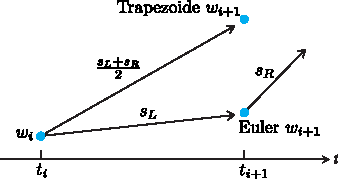
\includegraphics[width=.3\paperwidth]{trapezoid}
\end{figure}

La razón del nombre ``método del trapezoide'' es que en el caso especial donde
$f\left(t,y\right)$ es independiente de $y$, el método
\begin{equation*}
    w_{i+1}=
    w_{i}+
    \frac{h}{2}
    \left[
        f\left(t_{i}\right)+
        f\left(t_{i}+h\right)
        \right]
\end{equation*}
puede ser visto como añadir una aproximación de la regla del
trapezoide de la integral
\begin{math}
    \int_{t_{i}}^{t_{i}+h}
    f\left(t\right)\dl t
\end{math}
al actual $w_{i}$.
Dado que
\begin{equation*}
    \int_{t_{i}}^{t_{i}+h}
    f\left(t\right)\dl t=
    \int_{t_{i}}^{t_{i}+h}=
    \diff{y\left(t\right)}{t}\dl t=
    y\left(t_{i}+h\right)-y\left(t_{i}\right).
\end{equation*}
este corresponde a resolver la ecuación diferencial
$\diff{y}{t}=f\left(t\right)$ integrando ambos lados con el uso de
la regla del trapezoide.
\begin{equation*}
    \int_{x_{0}}^{x_{1}}
    f\left(x\right)
    \dl x=
    \frac{h}{2}\left(y_{0}+y_{1}\right)-
    \frac{h^{3}}{12}f^{\prime\prime}\left(c\right),
\end{equation*}
donde $h=x_{1}-x_{0}$ y $c$ está entre $x_{0}$ y $x_{1}$.
El método del trapezoide explícito también se denomina método de
Euler mejorado y método de Heun en la literatura.

\begin{questions}
    \question

    Calcule la aproximación del método del trapezoide en el intervalo
    $[0,1]$ para el problema de valor inicial $\diff{y}{t}=ty^{2}$,
    $y\left(0\right)=-1$ para un tamaño de paso $h=\frac{1}{4}$.
    Encuentre el error en $t=1$ comparando con la solución exacta
    \begin{math}
        y\left(t\right)=
        \frac{-2}{t^{2}+2}
    \end{math}.

    \question

    Dibuje la aproximación del método del trapezoide a la solución
    del problema de valor inicial
    \begin{equation*}
        \left\{
        \begin{aligned}
            \diff{y}{t}     & =
            3t^{2}y+4t^{2}.     \\
            y\left(0\right) & =
            5.
        \end{aligned}
        \right.
    \end{equation*}
    en el intervalo $\left[0,1\right]$ con tamaño de paso $h=0.1$,
    junto con la solución exacta
    \begin{math}
        y\left(t\right)=
        -\frac{4}{3}+
        \frac{19}{3}e^{t^{3}}
    \end{math}.

    \question

    Usando la condición inicial $y\left(0\right)=0$ y el tamaño de
    paso $h=\frac{1}{4}$, calcule la aproximación del método del
    trapezoide sobre el intervalo $\left[0,1\right]$.
    Encuentre el error en $t=1$.

    \begin{multicols}{3}
        \begin{parts}
            \part

            \begin{math}
                \diff{y}{t}=
                t+y
            \end{math}.

            \part

            \begin{math}
                \diff{y}{t}=
                t-y
            \end{math}.

            \part

            \begin{math}
                \diff{y}{t}=
                4t-2y
            \end{math}.
        \end{parts}
    \end{multicols}

    \question

    Calcule la solución aproximada del método del trapezoide en $\left[0,4\right]$
    para la ecuación diferencial $\diff{y}{t}=\operatorname{sen}\left(y\right)$
    y la condición inicial $y_{0}=100$, usando los tamaños de paso
    $h=0.1\times 2^{-k}$ para $0\leq k\leq 5$.
    Grafique las soluciones aproximadas $k=0$ y $k=5$ junto con la
    solución exacta (vea Exercise 6.1.15), and make a log–log plot of the error at t = 4 as a function of h.
\end{questions}

\subsection{Método de Taylor}

El método de Euler es de orden uno y el método del trapecio,
aparentemente superior, es de orden dos.
En esta sección, mostramos que existen métodos de todos los órdenes.
Para cada entero positivo $k$, existe un método de Taylor de orden
$k$, que describiremos a continuación.

La idea básica es una explotación directa de la expansión de Taylor.
Supongamos que la solución $y\left(t\right)$ es $\left(k+1\right)$
veces continuamente diferenciable.
Dado el punto actual $\left(t,y\left(t\right)\right)$ en la curva
solución, el objetivo es expresar $y\left(t+h\right)$ en términos de
$y\left(t\right)$ para un tamaño de paso $h$, utilizando información
sobre la ecuación diferencial.
La expansión de Taylor de $y\left(t\right)$ alrededor de $t$ es
\begin{equation*}
    y\left(t+h\right)=
    y\left(t\right)+
    h\diff{y\left(t\right)}{t}+
    \frac{h^{2}}{2}
    \diff[2]{y\left(t\right)}{t}+
    \cdots+
    \frac{h^{k}}{k!}
    \diff[k]{y\left(t\right)}{t}+
    \frac{h^{k+1}}{\left(k+1\right)!}
    \diff[k+1]{y\left(c\right)}{t},
\end{equation*}
donde $c$ se encuentra entre $t$ y $t+h$.
El último término es el término restante de Taylor.
Esta ecuación motiva el siguiente método:

\begin{align*}
    w_{0}   & =y_{0}  \\
    w_{i+1} & =w_{i}+
    h
    f\left(t_{i},w_{i}\right)+
    \frac{h^{2}}{2}
    \diff{f\left(t_{i},w_{i}\right)}{t}+
    \cdots+
    \frac{h^{k}}{k!}
    \diff[k-1]{f\left(t_{i},w_{i}\right)}{t}.
\end{align*}

\begin{questions}
    \question

    Encuentra la fórmula para el método de Taylor de segundo orden
    para las siguientes ecuaciones diferenciales

    \begin{multicols}{4}
        \begin{parts}
            \part

            \begin{math}
                \diff{y}{t}=
                ty
            \end{math}.

            \part

            \begin{math}
                \diff{y}{t}=
                ty^2+
                y^3
            \end{math}.

            \part

            \begin{math}
                \diff{y}{t}=
                y\operatorname{sen}\left(y\right)
            \end{math}.

            \part

            \begin{math}
                \diff{y}{t}=
                e^{yt^2}
            \end{math}.
        \end{parts}
    \end{multicols}

    \question

    Aplique el método de Taylor de segundo orden a los problemas de
    valor inicial del Ejercicio~\ref{question:first}.
    Utilizando el tamaño de paso $h=\frac{1}{4}$, calcule la
    aproximación del método de Taylor de segundo orden en el
    intervalo $\left[0,1\right]$.
    Compárelo con la solución correcta y encuentre el error en $t=1$.
\end{questions}

\subsection{Métodos de Runge-Kutta}

Los métodos de Runge-Kutta son una familia de solucionadores de EDOs
que incluyen los métodos de Euler y del trapezoide, así como métodos
más sofisticados de orden superior.
Un ejemplo importante es el método del punto medio.
\begin{align*}
    w_{0}   & =y_{0}                                                                             \\
    w_{i+1} & =w_{i}+hf\left(t_{i}+\frac{h}{2},w_{i}+\frac{h}{2}f\left(t_{i},w_{i}\right)\right)
\end{align*}
Para verificar el orden de convergencia del método del punto medio,
debemos calcular su error de truncamiento local.
Por un lado tenemos que
\begin{equation}\label{eq:taylorhelper}
    y_{i+1}=y_{i}+hf\left(t_{i},y_{i}\right)+
    \frac{h^{2}}{2}
    \left(
    \diffp{f\left(t_{i},y_{i}\right)}{t}+
    \diffp{f\left(t_{i},y_{i}\right)}{y}
    f\left(t_{i},y_{i}\right)
    \right)+
    \frac{h^{3}}{6}y^{\prime\prime\prime}\left(c\right).
\end{equation}
Para calcular el error de truncamiento local en el paso $i$,
suponemos que $w_{i}=y_{i}$ y calculamos $y_{i+1}-w_{i+1}$.
Repitiendo el uso de la expansión de la serie de Taylor como para
el método del trapezoide, podemos escribir
\begin{align}
    w_{i+1} & =
    y_{i}+hf\left(t_{i}+\frac{h}{2},y_{i}+\frac{h}{2}f\left(t_{i},y_{i}\right)\right) \notag \\
            & =
    y_{i}+
    h
    \left(
    f\left(t_{i},y_{i}\right)+
    \frac{h}{2}\diffp{f\left(t_{i},y_{i}\right)}{t}+
    \frac{h}{2}f\left(t_{i},y_{i}\right)
    \diffp{f\left(t_{i},y_{i}\right)}{y}+
    \mathcal{O}\left(h^{2}\right)
    \right).\label{eq:taylorhelper2}
\end{align}

Comparando~\eqref{eq:taylorhelper} y~\eqref{eq:taylorhelper2} se
obtiene
\begin{equation*}
    y_{i+1}-w_{i+1}=\mathcal{O}\left(h^{3}\right),
\end{equation*}
por lo tanto, el método del punto medio es de orden dos.
Cada evaluación de la función del lado derecho de la ecuación
diferencial se denomina etapa del método.
Los métodos del trapezoide y del punto medio son miembros de la
familia de métodos de Runge-Kutta de dos etapas y de segundo orden,
que tienen la forma
\begin{equation*}
    w_{i+1}=
    w_{i}+
    h\left(1-\frac{1}{2\alpha}\right)
    f\left(t_{i},w_{i}\right)+
    \frac{h}{2\alpha}
    f\left(t_{i}+\alpha h,w_{i}+\alpha hf\left(t_{i},w_{i}\right)\right)
\end{equation*}
para algún $\alpha\neq 0$.
Haciendo $\alpha=1$ corresponde al método del trapezoide explícito y
para $\alpha=\frac{1}{2}$ se obtiene el método del punto medio.

\begin{figure}[ht!]
    \centering
    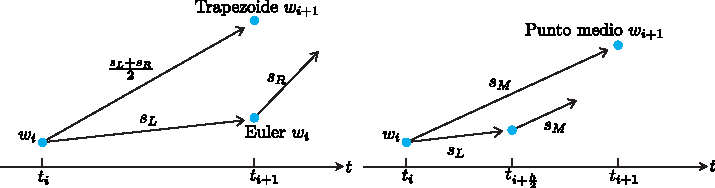
\includegraphics[width=.6\paperwidth]{midpoint}
\end{figure}

El método del trapezoide utiliza un paso de Euler hasta el extremo
derecho del intervalo, evalúa la pendiente allí y luego promedia con
la pendiente desde el extremo izquierdo.
El método del punto medio utiliza un paso de Euler para moverse hasta
el punto medio del intervalo, evalúa la pendiente allí como
\begin{math}
    f
    \left(
    t_{i}+\frac{h}{2},
    w_{i}+\frac{h}{2}
    f\left(t_{i},w_{i}\right)
    \right)
\end{math},
y utiliza esa pendiente para moverse desde $w_{i}$ hasta la nueva
aproximación $w_{i+1}$.
Estos métodos utilizan diferentes enfoques para resolver el mismo
problema: adquirir una
pendiente que represente todo el intervalo mejor que el método de
Euler, que utiliza solo la estimación de la pendiente desde el
extremo izquierdo del intervalo.

\begin{align*}
    w_{i+1} & =
    w_{i}+
    \frac{h}{6}
    \left(s_{1}+2s_{2}+2s_{3}+s_{4}\right).                 \\
    s_{1}   & =
    f\left(t_{i},w_{i}\right).                              \\
    s_{2}   & =
    f\left(t_{i}+\frac{h}{2},w_{i}+\frac{h}{2}s_{1}\right). \\
    s_{3}   & =
    f\left(t_{i}+\frac{h}{2},w_{i}+\frac{h}{2}s_{2}\right). \\
    s_{4}   & =
    f\left(t_{i}+h,w_{i}+hs_{3}\right).
\end{align*}

La popularidad de este método se debe a su simplicidad y facilidad de programación.
Es un método de un solo paso, por lo que solo requiere una condición
inicial para comenzar; sin embargo, como método de cuarto orden, es
considerablemente más preciso que los métodos de Euler o del
trapezoide.

La cantidad $\frac{h}{6}\left(s_{1}+2s_{2}+2s_{3}+s_{4}\right)$ en el
método de Runge-Kutta de cuarto orden reemplaza a la pendiente en el
método de Euler.
Esta cantidad puede considerarse como una estimación mejorada de la
pendiente de la solución en el intervalo $\left[t_{i},t_{i}+h\right]$.
Nótese que $s_{1}$ es la pendiente en el extremo izquierdo del intervalo,
$s_{2}$ es la pendiente utilizada en el método del punto medio,
$s_{3}$ es una pendiente mejorada en el punto medio y $s_{4}$ es una
pendiente aproximada en el punto extremo derecho $t_{i}+h$.

\begin{questions}
    \question

    Aplique el método del punto medio para los problemas de valor inicial

    \begin{multicols}{3}
        \begin{parts}
            \part

            \begin{math}
                \diff{y}{t}=
                t
            \end{math}.

            \part

            \begin{math}
                \diff{y}{t}=
                t^{2}y
            \end{math}.

            \part

            \begin{math}
                \diff{y}{t}=
                2\left(t+1\right)y
            \end{math}

            \part

            \begin{math}
                \diff{y}{t}=
                5t^{4}y
            \end{math}.

            \part

            \begin{math}
                \diff{y}{t}=
                \frac{1}{y^{2}}
            \end{math}.

            \part

            \begin{math}
                \diff{y}{t}=
                \frac{t^{3}}{y^{2}}
            \end{math}.
        \end{parts}
    \end{multicols}
    with initial condition $y\left(0\right)=1$.
    Utilizando el tamaño de paso $h=\frac{1}{4}$, calcule la
    aproximación del método del punto medio en el intervalo
    $\left[0,1\right]$.
    Compare con la solución correcta y encuentre el error de
    truncamiento global en $t=1$.

    \question

    Aplique el método de Runge-Kutta de cuarto orden a los problemas
    de valor inicial en el ejercicio anterior.
    Usando el tamaño de paso $h=\frac{1}{4}$, calcule la aproximación
    en el intervalo $\left[0,1\right]$.
    Compare con la solución correcta y encuentre el error de
    truncamiento global en $t=1$.

    \question

    Asuma que el lado derecho $f\left(t,y\right)=f\left(t\right)$ no depende de $y$.
    Muestre que $s_{2}=s_{3}$ en Runge-Kutta de cuarto orden y que
    RK4 es equivalente a la regla de Simpson para la integral
    \begin{math}
        \int_{t_{i}}^{t_{i}+h}
        f\left(s\right)
        \dl s
    \end{math}.

    \question

    Grafique la solución aproximada del método de Runge-Kutta de
    cuarto orden en $\left[0,1\right]$ para la ecuación diferencial
    $\diff{y}{t}=1-y^{2}$ y la condición inicial
    $y_{0}=-\frac{1}{2}$, junto con la solución exacta.
    Use tamaños de paso $h=0.1$ y $0.05$.
\end{questions}

\subsection{Método de Euler implícito}

Los solucionadores de ecuaciones diferenciales que hemos presentado
hasta ahora son explícitos, lo que significa que existe una fórmula
explícita para la nueva aproximación $w_{i+1}$ en términos de datos
conocidos, como $h$, $t_{i}$ y $w_{i}$.
Resulta que algunas ecuaciones diferenciales no se resuelven
adecuadamente con métodos explícitos, y nuestro primer objetivo es
explicar por qué.

Las ecuaciones diferenciales con esta propiedad (que las soluciones
atractivas están rodeadas de soluciones cercanas que cambian
rápidamente) se denominan rígidas.

\begin{align*}
    w_{0}   & =
    y_{0}.      \\
    w_{i+1} & =
    w_{i}+hf\left(t_{i+1},w_{i+1}\right).
\end{align*}

Debido al mejor comportamiento de los métodos implícitos como el
método de Euler hacia atrás en presencia de ecuaciones rígidas, vale
la pena realizar un trabajo adicional para evaluar el siguiente paso,
aunque no esté disponible explícitamente.
Si el método implícito deja una ecuación no lineal para resolver,
tanto la iteración de punto fijo como el método de Newton se
utilizan a menudo para resolver $w_{i+1}$.
Esto significa que hay un bucle de resolución de ecuaciones dentro
del bucle que avanza la ecuación diferencial.

\begin{questions}
    \question

    Utilizando la condición inicial $y\left(0\right)=1$ y el tamaño
    del paso $h=\frac{1}{4}$, calcule la aproximación de Euler hacia
    atrás a $\diff{y}{t}=ty$ en el intervalo $\left[0,1\right]$.
    Encuentre el error en $t=1$ comparando con la solución exacta.

    \question

    Aplique el método de Euler hacia atrás, utilizando el método de
    Newton como solucionador, para los problemas de valor inicial.
    ¿Cuál de las soluciones de equilibrio se alcanza con la solución
    aproximada?
    Aplique el método de Euler.
    ¿Para qué rango aproximado de $h$ se puede utilizar Euler con
    éxito para converger al equilibrio?
    Grafique las soluciones aproximadas dadas por Euler hacia atrás y
    por Euler con un tamaño de paso excesivo.

    \begin{multicols}{2}
        \begin{parts}
            \part

            \begin{equation*}
                \left\{
                \begin{aligned}
                    \diff{y}{t}     & =y^{2}-y^{3},\quad t\in\left[0,20\right] \\
                    y\left(0\right) & =\frac{1}{2}
                \end{aligned}
                \right.
            \end{equation*}

            \part

            \begin{equation*}
                \left\{
                \begin{aligned}
                    \diff{y}{t}     & =y^{2}-y^{3},\quad t\in\left[0,20\right] \\
                    y\left(0\right) & =\frac{1}{2}
                \end{aligned}
                \right.
            \end{equation*}
        \end{parts}

    \end{multicols}
\end{questions}

\subsection{Métodos multipasos}

La familia Runge-Kutta que hemos estudiado consta de métodos de un
solo paso, lo que significa que el paso más nuevo $w_{i+1}$ se
produce sobre la base de la ecuación diferencial y el valor del paso
anterior $w_{i}$.
Los métodos de múltiples pasos sugieren un enfoque diferente: usar el
conocimiento de más de uno de los $w_{i}$ anteriores para ayudar a
producir el siguiente paso.
Esto conducirá a solucionadores de EDO que tienen un orden tan alto
como los métodos de un solo paso, pero gran parte del cálculo
necesario se reemplazará con la interpolación de valores ya
calculados en la ruta de la solución.

\subsubsection{Método de Adams-Bashforth de dos pasos}

Considere el siguiente método de dos pasos que es de segundo orden:

\begin{equation*}
    w_{i+1}=
    w_{i}+h\left[\frac{3}{2}f\left(t_{i},w_{i}\right)-\frac{1}{2}f\left(t_{i-1},w_{i-1}\right)\right].
\end{equation*}

El método de dos pasos Adams-Bashforth requiere solo una nueva
evaluación por paso (se almacena una del paso anterior).
Los métodos de varios pasos pueden lograr el mismo orden con menos
esfuerzo computacional (normalmente solo una evaluación de función por paso).
Dado que los métodos de varios pasos utilizan más de un valor $w$
previo, necesitan ayuda para comenzar.
La fase de inicio de un método de $s$ pasos generalmente consiste en
un método de un solo paso que utiliza $w_{0}$ para producir $s-1$
valores $w_{1},w_{2},\dotsc,w_{s−1}$, antes de que se pueda utilizar
el método de varios pasos.
El método de dos pasos de Adams-Bashforth necesita $w_{1}$, junto con
la condición inicial dada $w_{0}$, para comenzar.

\begin{listing}[ht!]
    \tiny
    \centering
    \inputminted[linenos,highlightlines={7-24}]{octave}{exmultistep.m}
    \inputminted[linenos,highlightlines={1-8}]{octave}{trapstep.m}
    \inputminted[linenos,highlightlines={1-5}]{octave}{ab2step.m}
    \inputminted[linenos,highlightlines={1-5}]{octave}{unstable2step.m}
    \inputminted[linenos,highlightlines={1-5}]{octave}{weaklystable2step.m}
    \inputminted[linenos,highlightlines={1-4}]{octave}{ydot.m}
    \caption{Método de Adams-Bashforth.}
\end{listing}

El método general de $s$ pasos tiene la forma
\begin{equation*}
    w_{i+1}=
    a_{1}w_{i}+
    a_{2}w_{i−1}+\cdots+
    a_{s}w_{i-s+1}+
    h\left[
    b_{0}f_{i+1}+
    b_{1}f_{i}+
    b_{2}f_{i-1}+
    \cdots+
    b_{s}f_{i-s+1}\right].
\end{equation*}

El tamaño de paso es $h$, y usamos la notación
\begin{equation*}
    f_{i}\equiv
    f\left(t_{i},w_{i}\right).
\end{equation*}
Si $b_{0}=0$, el método es explícito, caso contrario, el método es
implícito.

\subsubsection{Método de Adams-Moulton de dos pasos (tercer orden)}

\begin{equation*}
    w_{i+1}=
    w_{i}+
    \frac{h}{12}\left[5f_{i+1}+8f_{i}-f_{i-1}\right].
\end{equation*}

\subsubsection{Método de Adams-Moulton de tres pasos (cuarto orden)}

\begin{equation*}
    w_{i+1}=
    w_{i}+
    \frac{h}{24}\left[9f_{i+1}+19f_{i}-5f_{i-1}+f_{i-2}\right].
\end{equation*}

\subsubsection{Método de Adams-Moulton de cuatro pasos (quinto orden)}

\begin{equation*}
    w_{i+1}=
    w_{i}+
    \frac{h}{720}\left[251f_{i+1}+646f_{i}-264f_{i-1}+106f_{i-2}-19f_{i-3}\right].
\end{equation*}

Estos métodos se utilizan ampliamente en métodos
predictores-correctores, junto con un predictor Adams-Bashforth del
mismo orden.

\begin{listing}[ht!]
    \tiny
    \centering
    \inputminted[linenos,highlightlines={8-31}]{octave}{predcorr.m}
    \inputminted[linenos,highlightlines={1-5}]{octave}{am1step.m}
    \caption{Método de Adams-Moulton.}
\end{listing}

\begin{questions}
    \question


    Aplique el método de dos pasos de Adams-Bashforth a los problemas de valor inicial

    \begin{multicols}{3}

        \begin{parts}
            \part

            \begin{math}
                \diff{y}{t}=t
            \end{math}.

            \part

            \begin{math}
                \diff{y}{t}=t^{2}y
            \end{math}.

            \part

            \begin{math}
                \diff{y}{t}=2\left(t+1\right)y
            \end{math}.

            \part

            \begin{math}
                \diff{y}{t}=5t^{4}y
            \end{math}.

            \part

            \begin{math}
                \diff{y}{t}=
                \frac{1}{y^{2}}
            \end{math}.

            \part

            \begin{math}
                \diff{y}{t}=
                \frac{t^{3}}{y^{2}}
            \end{math}.
        \end{parts}
    \end{multicols}
    con la condición inicial $y\left(0\right)=1$.
    Utilice un tamaño de paso $h=\frac{1}{4}$ en el intervalo
    $\left[0,1\right]$.
    Utilice el método del trapezoide explícito para crear $w_{1}$.
    Encuentre el error de truncamiento global en $t=1$.

    \question

    Encuentre un método explícito de dos pasos y segundo orden cuyo
    polinomio característico tenga una raíz doble en $1$.

    \question

    Encuentre el orden y el tipo de estabilidad para los siguientes
    métodos implícitos de dos pasos:

    \begin{parts}
        \part

        \begin{math}
            w_{i+1}=
            3w_{i}-2w_{i-1}+\frac{h}{12}\left[13f_{i+1}-20f_{i}-5f_{i-1}\right]
        \end{math}.

        \part

        \begin{math}
            w_{i+1}=
            \frac{4}{3}w_{i}-\frac{1}{3}w_{i-1}+\frac{2}{3}hf_{i+1}
        \end{math}.

        \part

        \begin{math}
            w_{i+1}=
            \frac{4}{3}w_{i}-
            \frac{1}{3}w_{i-1}+
            \frac{h}{9}
            \left[4f_{i+1}+4f_{i}-2f_{i-1}\right]
        \end{math}.

        \part

        \begin{math}
            w_{i+1}=
            3w_{i}-2w_{i-1}+
            \frac{h}{12}\left[7f_{i+1}-8f_{i}-11f_{i-1}\right]
        \end{math}.

        \part

        \begin{math}
            w_{i+1}=
            2w_{i}-
            w_{i-1}+
            \frac{h}{2}
            \left[f_{i+1}-f_{i-1}\right]
        \end{math}.
    \end{parts}

    \question

    Adapte el programa \mintinline{bash}|exmultistep.m| para aplicar
    el método de dos pasos de Adams-Bashforth a los problemas de
    valor inicial del ejercicio anterior.
    Con un tamaño de paso $h=0.1$, calcule la aproximación en el
    intervalo $\left[0,1\right]$.
    Imprima una tabla de los valores $t$, las aproximaciones y el
    error de truncamiento global en cada paso.

    \question

    Grafique la solución aproximada del método Adams-Bashforth de
    tres pasos en $\left[0,1\right]$ para la EDO $\diff{y}{t}=1-y^{2}$
    y la condición inicial $y_{0}=-\frac{1}{2}$, junto con la solución exacta.
    Use tamaños de paso $h=0.1$ y $0.05$.

    \question

    Calcule la solución aproximada del método de tres pasos de
    Adams-Bashforth de la ecuación diferencial
    $\diff{y}{t}=\operatorname{senh}\left(y\right)$ y la condición
    inicial $y_{0}=\frac{1}{4}$ en el intervalo $\left[0, 2\right]$.
    Utilizando tamaños de paso $h=0.1\times 2^{-k}$ para $0\leq k\leq 5$.
    Grafique las soluciones aproximadas $k=0$ y $k=5$ junto con la
    solución exacta y haga un gráfico logarítmico del error en función de $h$.
\end{questions}

\providecommand{\name}{Nombre}
\vfill{Nombre}\footnote{Hecho en \LaTeX}
\hfill{UNI, 12 de febrero de 2025}

\end{document}